\chapter{薄板伽辽金无网格法} 
\section{伽辽金无网格离散}
考虑如图(\ref{plate})所示薄板区域$\bar \Omega$,其中板厚为$h$,$\Omega$为薄板中面。根据Kirchhoff薄板假设原理[],在薄板中面$\Omega$上的控制方程为:
\begin{equation}
    \begin{cases}\label{P control equation}
        M_{\alpha\beta,\alpha\beta}+\bar q=0&\mathrm{in} \; \Omega\\
        w=\bar w&\mathrm{on}\;\Gamma_w\\
        \theta_{\pmb n}=w_{,\pmb n}=\bar \theta_{\pmb n}&\mathrm{on}\;\Gamma_{\theta}\\
        V_{\pmb n}=Q_{\pmb n}+M_{\pmb{ns},\pmb s}=\bar V_{\pmb n}&\mathrm{on}\;\Gamma_V\\
        M_{\pmb{nn}}=\bar M_{\pmb{nn}}&\mathrm{on}\; \Gamma_M\\
        w=\bar w&\mathrm{at} \; c_w\\
        P=-M_{ns}\vert_{c_p}=\bar p&\mathrm{at}\; c_P
    \end{cases}
\end{equation}
\begin{figure}[!h]
    \centering
    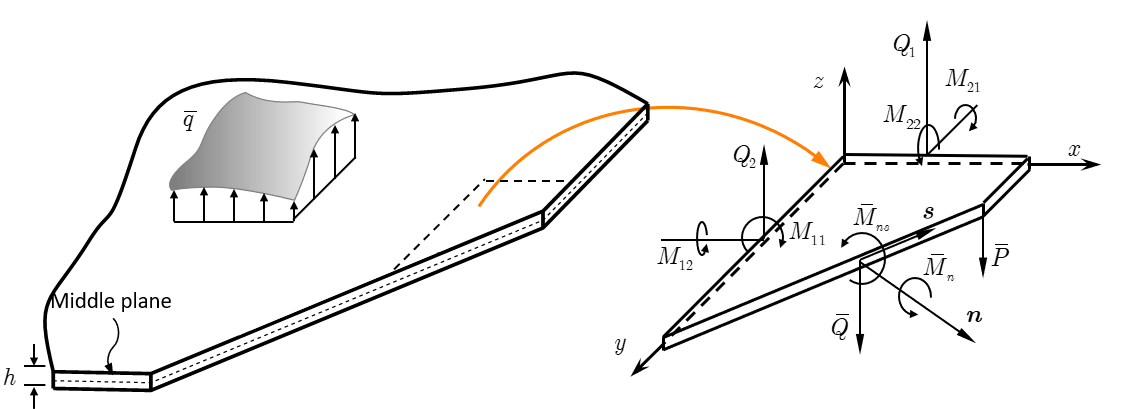
\includegraphics[scale=0.7]{figure/P/plate.png}
    \caption{薄板运动学及边界条件}\label{plate}
\end{figure}
其中式(\ref{P control equation})存在如下关系式:
\begin{align}
\label{wn} &w_{,\pmb n}=w_{,\alpha}n_{\alpha}\\
\label{Qn} &Q_{\pmb n}=n_{\alpha}M_{\alpha\beta,\beta}\\
\label{Mn} &M_{\pmb{nn}}=M_{\alpha\beta}n_{\alpha}n_{\beta},M_{\pmb{ns}}=M_{\alpha\beta n_{\alpha}s_{\beta}},M_{\pmb{ns,s}}=M_{\alpha\beta,\gamma}s_{\alpha}n_{\beta}s_{\gamma}
\end{align}
式中$M_{\alpha\beta}$为矩量$\boldsymbol M$的弯曲和扭转分量,$\bar q$为垂直于薄板中面的分布荷载。$\Gamma_w$、$\Gamma_{\theta}$和$c_w$为本质边界条件,$\bar w$和$\bar \theta_n$分别为本质边界条件上给定的挠度和转角。
$\Gamma_V$、$\Gamma_M$和$c_P$为自然边界条件,$V_{\boldsymbol n}$、$M_{\boldsymbol{nn}}$和$P$为自然边界上的等效剪力、法向弯矩和薄板角上的集中荷载。$\pmb{n}=\{n_x,\; n_y\}^T$,$\pmb{s}=\{s_x,\; s_y\}^T$分别表示所在边界方向上的外法线方向和切方向的分量。
所有的边界条件都满足如下关系式:
\begin{equation}\label{PGeometric relationships}
    \begin{split}
        \Gamma=\Gamma_w\cup\Gamma_V\cup\Gamma_{\theta}\cup\Gamma_M,c=c_w\cup c_P\\
        \Gamma_w\cap\Gamma_V=\Gamma_{\theta}\cap\Gamma_M=c_w\cap c_P=\varnothing
    \end{split}
\end{equation}\par
当薄板为线弹性各同向性材料时,其本构关系表达式如下:
\begin{equation}
    \begin{split}\label{Malphabeta}
        M_{\alpha\beta}=D_{\alpha\beta\gamma\eta}\kappa_{\gamma\eta}=-D_{\alpha\beta\gamma\eta}w_{,\gamma\eta}
    \end{split}
\end{equation}
其中:
\begin{equation}
    \begin{split}\label{Dalphabeta}
        D_{\alpha\beta\gamma\eta}=\bar D(\nu\delta_{\alpha\beta}\delta_{\gamma\eta}+\frac{1}{2}(1-\nu)(\delta_{\alpha\gamma}\delta_{\beta\eta}+\delta_{\alpha\gamma}\delta_{\beta\gamma}))
    \end{split}
\end{equation}
式中,$\kappa_{\alpha\beta}=-w_{,\alpha\beta}$为曲率张量$\boldsymbol \kappa$的分量。$D_{\alpha \beta \gamma \eta}$为四阶弹性张量,$\bar{D}$分为抗弯刚度,其可采用杨氏模量$E$、泊松比$\nu$和板厚$h$表示为:
\begin{equation}\label{kangwangangdu}
    \begin{split}
    \bar D=\frac{Eh^3}{12(1-\nu^2)}
\end{split}
\end{equation}\par
根据尺寸相关弹性[],此时将式(\ref{Qn})、(\ref{Mn})、(\ref{Malphabeta})、(\ref{Dalphabeta})代入式(\ref{P control equation})中可以得到自然边界上的法向弯矩$M_{\pmb{nn}}$、等效剪力$V_{\pmb{n}}$和薄板角上的集中荷载$P$的具体表达式:
\begin{equation}
\begin{split}\label{MVP}
    \begin{cases}
        M_{\pmb{nn}}=\mathcal{M}_{\alpha\beta}w_{,\alpha\beta}=-\bar{D}(\nu\delta_{\alpha\beta}+(1-\nu)n_{\alpha}n_{\beta})w_{,\alpha\beta}\\
        V_{\pmb{n}}=\mathcal{V}_{\alpha\beta}w_{,\alpha\beta}=-\bar{D}(\frac{\partial}{\partial x_{\alpha}}n_{\beta}+(1-\nu)n_{\alpha}\frac{\partial}{\partial y_{\gamma}}s_{\alpha}n_{\beta}s_{\gamma})w_{,\alpha\beta}\\
        P=\mathcal{P}_{\alpha\beta}w_{,\alpha\beta}=-[[(\bar{D}(1-\nu)n_{\alpha}s_{\beta})w_{,\alpha\beta}]]
    \end{cases}
\end{split}
\end{equation}
其中:
\begin{equation}
\begin{split}\label{MVP1}
    \begin{cases}
 \mathcal{M}_{\alpha\beta}w_{,\alpha\beta}=-D_{\alpha\beta\gamma\eta}n_{\gamma}n_{\eta}=-\bar{D}(\nu\delta_{\alpha\beta}+(1-\nu)n_{\alpha}n_{\beta})\\
  \mathcal{V}_{\alpha\beta}w_{,\alpha\beta}=-D_{\alpha\beta\gamma\eta}(n_{\gamma}\frac{\partial}{\partial x_{\eta}}+s_{\gamma}n_{\eta}s_{\xi}\frac{\partial}{\partial x_{\xi}})=-\bar{D}(\frac{\partial}{\partial x_{\alpha}}n_{\beta}+(1-\nu)n_{\alpha}\frac{\partial}{\partial y_{\gamma}}s_{\alpha}n_{\beta}s_{\gamma})\\
 \mathcal{P}_{\alpha\beta}w_{,\alpha\beta}=-[[D_{\alpha\beta}n_{\gamma}s_{\eta}]]=-[[\bar{D}(1-\nu)n_{\alpha}s_{\beta}]]
    \end{cases}
\end{split}
\end{equation}
根据最小势能原理,式(\ref{P control equation})的势能泛函表达式为:
\begin{equation}\label{Pshineng}
\begin{split}
    \Pi(w)&=\int_{\Omega}\frac{1}{2}\kappa_{,\alpha\beta}M_{\alpha\beta}d\Omega+\int_{\Gamma_M}\theta_{\pmb{n}}\bar{M}_{\pmb{nn}}d\Gamma\\
    &-\int_{\Gamma_V}w\bar{V}_{\pmb{n}}d\Gamma-w\bar{P}\vert_{x\in c_P}+\int_{\Omega}w\bar{q}d\Omega
\end{split}
\end{equation}
对式(\ref{Pshineng})进行变分得到四阶薄板问题的伽辽金弱形式:
\begin{equation}\label{Pweakform}
\begin{split}
        \delta\Pi(w)&=\int_{\Omega}\delta\kappa_{,\alpha\beta}M_{\alpha\beta}d\Omega+\int_{\Gamma_M}\delta\theta_{\pmb{n}}\bar{M}_{\pmb{nn}}d\Gamma\\
        &-\int_{\Gamma_V}\delta w\bar{V}_{\pmb{n}}d\Gamma-\delta w\bar{P}\vert_{x\in c_P}+\int_{\Omega}\delta w\bar{q}d\Omega
\end{split}
\end{equation}
引入无网格离散:
\begin{equation}
\begin{split}\label{Pwuwangelisan}
    w^h(\pmb{x})=\sum_{I=1}^{N\!P}\Psi_I(\pmb{x})d_I \;\delta w^h(\pmb{x})=\sum_{I=1}^{N\!P}\Psi_I(\pmb{x})\delta d_I\\
\end{split}
\end{equation}
将式(\ref{Pwuwangelisan})代入$\kappa_{\alpha\beta}=-w_{,\alpha\beta}$得到离散的曲率张量:
\begin{equation}
\begin{split}
\pmb{\kappa}=\sum_{I=1}^{N\!P}\pmb{B}_I(\pmb{x})\pmb{d}_I\;
\pmb{B}_I(\pmb{x})= \left[\begin{matrix}\Psi_{I,xx}\\\Psi_{I,yy}\\2\Psi_{I,xy}\end{matrix}\right] 
\end{split}
\end{equation}
将式(\ref{wn})、(\ref{Malphabeta})和(\ref{Pwuwangelisan})代入到弱形式(\ref{Pweakform})中得到薄板问题伽辽金无网格法离散平衡控制方程:
\begin{equation}
\begin{split}
    \delta\pmb{d}(\pmb{K}\pmb{d}&-\pmb{f})=0\\
     &\pmb{K}\pmb{d}=\pmb{f}
\end{split}
\end{equation}
其中:
\begin{equation}
\begin{split}
    K_{IJ}=\int_{\Omega}\pmb{B}^T_I\pmb{D}\pmb{B}_Jd\Omega
\end{split}
\end{equation}
\begin{equation}
\begin{split}
    f_I=\int_{\Gamma_V}\Psi_I\bar{V}_{\pmb{n}}d\Gamma-\int_{\Gamma_M}\Psi_{I,\pmb{n}}\bar{M}_{\pmb{nn}}d\Gamma+\Psi_I\bar{P}\vert_{x\in C_P}+\int_{\Omega}\Psi_I\bar{q}d\Omega
\end{split}
\end{equation}
\section{强制边界条件施加方法}
\subsection{修正变分原理法}
根据[]修正变分原理法的薄板问题势能泛函表达式为:
\begin{equation}\label{Psigman}
\begin{split}
    \bar{\Pi}(w)&=\frac{1}{2}\int_{\Omega}\kappa_{,\alpha\beta}M_{\alpha\beta}d\Omega+\int_{\Gamma_M}\theta_{\pmb{n}}\bar{M}_{\pmb{nn}}d\Gamma-\int_{\Gamma_V}w\bar{V}_{\pmb{n}}d\Gamma-w\bar{P}\vert_{x\in c_P}+\int_{\Omega}w\bar{q}d\Omega\\
    &-\int_{\Gamma_w}V_{\pmb{n}}(w-\bar{w})d\Gamma+\int_{\theta}M_{\pmb{nn}}(\theta_{\pmb{n}}-\bar{\theta}_{\pmb{n}})d\Gamma-P(w-\bar{w})\vert_{x\in c_w}\\
\end{split}
\end{equation}
对式(\ref{Psigman})进行变分得到修正变分原理法的伽辽金弱形式为:
\begin{equation}
    \begin{split}
    &\int_{\Omega}\delta\kappa_{,\alpha\beta}M_{\alpha\beta}d\Omega-\int_{\Gamma_w}(\delta V_{\pmb{n}}w+\delta wV_{\pmb{n}})d\Gamma+\int_{\Gamma_{\theta}}(\delta M_{\pmb{nn}}\theta_{\pmb{n}}+\delta\theta_{\pmb{n}}M_{\pmb{nn}})d\Gamma\\
    &-(\delta Pw+\delta wP)\vert_{x\in c_w}
    =\int_{\Gamma_M}\delta\theta_{\pmb{n}}\bar{M}_{\pmb{nn}}d\Gamma-\int_{\Gamma_V}\delta w\bar{V}_{\pmb{n}}d\Gamma-\delta w\bar{P}\vert_{x\in c_P}\\
    &+\int_{\Omega}\delta w\bar{q}d\Omega
    -\int_{\Gamma_w}\delta V_{\pmb{n}}\bar{w}d\Gamma+\int_{\Gamma_{\theta}}\delta M_{\pmb{nn}}\bar{\theta}_{\pmb{n}}d\Gamma-\delta P\bar{w}\vert_{x\in c_w}
\end{split}
\end{equation}\par
引入无网格离散式(\ref{Pwuwangelisan})和式(\ref{wn})-(\ref{MVP1})得到修正变分原理法伽辽金无网格离散平衡控制方程:
\begin{equation}
\begin{split}
    (\pmb{K}+\pmb{K}^n)\pmb{d}=\pmb{f}+\pmb{f}^n
\end{split}
\end{equation}
其中:
\begin{equation}
\begin{split}
    &K_{IJ}=\int_{\Omega}\pmb{B}^T_I\pmb{D}\pmb{B}_Jd\Omega\\
    &f_I=\int_{\Gamma_V}\Psi_I\bar{V}_{\pmb{n}}d\Gamma-\int_{\Gamma_M}\Psi_{I,\pmb{n}}\bar{M}_{\pmb{nn}}d\Gamma+\Psi_I\bar{P}\vert_{x\in C_P}+\int_{\Omega}\Psi_I\bar{q}d\Omega
\end{split}
\end{equation}
\begin{equation}
\begin{split}
     K^n_{IJ}&=-\int_{\Gamma_w}\Psi_I\mathcal{V}_{\alpha\beta}\Psi_{J,\alpha\beta}d\Gamma+\int_{\Gamma_{\theta}}\Psi_{I,n}\mathcal{M}_{\alpha\beta}\Psi_{J,\alpha\beta}d\Gamma+[[\Psi_I\mathcal{P}_{\alpha\beta}\Psi_{J,\alpha\beta}]]_{x\in{c_w}}\\
     &-\int_{\Gamma_w}\mathcal{V}_{\alpha\beta}\Psi_{I,\alpha\beta}\Psi_Jd\Gamma+\int_{\Gamma_{\theta}}\mathcal{M}_{\alpha\beta}\Psi_{I,\alpha\beta}\Psi_{J,n}d\Gamma+[[\mathcal{P}_{\alpha\beta}\tilde{\Psi}_{I,\alpha\beta}\Psi_J]]_{x\in{c_w}}\\
     f_{I}^n&=-\int_{\Gamma_w}\mathcal{V}_{\alpha\beta}\Psi_{I,\alpha\beta}\bar{w}d\Gamma+\int_{\Gamma_{\theta}}\mathcal{M}_{\alpha\beta}\Psi_{I,\alpha\beta}\bar{\theta}_{\pmb n}d\Gamma+[[\mathcal{P}_{\alpha\beta}\Psi_{I,\alpha\beta}\bar{w}]]_{x\in{c_w}}
\end{split}
\end{equation}
\subsection{罚函数法}
根据[]通过引入罚因子$\alpha$得到罚函数法薄板问题势能泛函表达式为:
\begin{equation}\label{Ppenalty}
\begin{split}
        \bar{\Pi}(w)&=\frac{1}{2}\int_{\Omega}\kappa_{,\alpha\beta}M_{\alpha\beta}d\Omega+\int_{\Gamma_M}\theta_{\pmb{n}}\bar{M}_{\pmb{nn}}d\Gamma-\int_{\Gamma_V}w\bar{V}_{\pmb{n}}d\Gamma-w\bar{P}\vert_{x\in c_P}+\int_{\Omega}w\bar{q}d\Omega\\
    &+\frac{\alpha_w}{2}\int_{\Gamma_w}(w-\bar{w})^2d\Gamma+\frac{\alpha_{\theta}}{2}\int_{\Gamma_{\theta}}(\theta_{\pmb{n}}-\bar{\theta}_{\pmb{n}})^2d\Gamma+\frac{\alpha_c}{2}(w-\bar{w})^2\vert_{x\in c_w}
\end{split}
\end{equation}
对式(\ref{Ppenalty})进行变分得到罚函数法伽辽金弱形式为:
\begin{equation}
\begin{split}
    &\int_{\Omega}\delta\kappa_{,\alpha\beta}M_{\alpha\beta}d\Omega
    +\alpha_w\int_{\Gamma_w}\delta wwd\Gamma+\alpha_{\theta}\int_{\Gamma_{\theta}}\delta\theta_{\pmb{n}}\theta_{\pmb{n}}d\Gamma+\alpha_c\delta ww\vert_{x\in c_w}\\
    &=\int_{\Gamma_M}\delta\theta_{\pmb{n}}\bar{M}_{\pmb{nn}}d\Gamma-\int_{\Gamma_V}\delta w\bar{V}_{\pmb{n}}d\Gamma-\delta w\bar{P}\vert_{x\in c_P}+\int_{\Omega}\delta w\bar{q}d\Omega\\
    &+\alpha_w\int_{\Gamma_w}\delta w\bar{w}d\Gamma+\alpha_{\theta}\int_{\Gamma_{\theta}}\delta\theta_{\pmb{n}}\bar{\theta}_{\pmb{n}}d\Gamma+\alpha_c\delta w\bar{w}\vert_{x\in c_w}
\end{split}
\end{equation}\par
引入式(\ref{wn})、(\ref{Malphabeta})和(\ref{Pwuwangelisan})得到罚函数法伽辽金无网格离散平衡控制方程:
\begin{equation}
\begin{split}
    (\pmb{K}+\pmb{K}^{\alpha})\pmb{d}=\pmb{f}+\pmb{f}^{\alpha}
\end{split}
\end{equation}
其中:
\begin{equation}
\begin{split}
    &K_{IJ}=\int_{\Omega}\pmb{B}^T_I\pmb{D}\pmb{B}_Jd\Omega\\
    &f_I=\int_{\Gamma_V}\Psi_I\bar{V}_{\pmb{n}}d\Gamma-\int_{\Gamma_M}\Psi_{I,\pmb{n}}\bar{M}_{\pmb{nn}}d\Gamma+\Psi_I\bar{P}\vert_{x\in C_P}+\int_{\Omega}\Psi_I\bar{q}d\Omega
\end{split}
\end{equation}
\begin{equation}
\begin{split}
   &K^{\alpha}_{IJ}=\alpha_w\int_{\Gamma_w}\Psi_I\Psi_Jd\Gamma+\alpha_{\theta}\int_{\Gamma_{\theta}}\Psi_{I,\pmb n}\Psi_{J,\pmb n}d\Gamma+\alpha_c\Psi_I\Psi_J\vert_{x\in c_w}\\
&f^{\alpha}_I=\alpha_w\int_{\Gamma_w}\Psi_I\bar{w}d\Gamma+\alpha_{\theta}\int_{\Gamma_{\theta}}\Psi_{I,\pmb n}\bar{\theta}_{\pmb n}d\Gamma+\alpha_c\Psi_I\bar{w}\vert_{x\in c_w}
\end{split}
\end{equation}
\subsection{Nitsche法}
Nitsche法是结合修正变分原理法和罚函数法,薄板问题的泛函表达式为:
\begin{equation}\label{Pnitsche}
\begin{split}
    \bar{\Pi}(w)&=\frac{1}{2}\int_{\Omega}\kappa_{,\alpha\beta}M_{\alpha\beta}d\Omega+\int_{\Gamma_M}\theta_{\pmb{n}}\bar{M}_{\pmb{nn}}d\Gamma-\int_{\Gamma_V}w\bar{V}_{\pmb{n}}d\Gamma-w\bar{P}\vert_{x\in c_P}+\int_{\Omega}w\bar{q}d\Omega\\
&-\int_{\Gamma_w}V_{\pmb{n}}(w-\bar{w})d\Gamma+\int_{\theta}M_{\pmb{nn}}(\theta_{\pmb{n}}-\bar{\theta}_{\pmb{n}})d\Gamma-P(w-\bar{w})\vert_{x\in c_w}\\
&+\frac{\alpha_w}{2}\int_{\Gamma_w}(w-\bar{w})^2d\Gamma+\frac{\alpha_{\theta}}{2}\int_{\Gamma_{\theta}}(\theta_{\pmb{n}}-\bar{\theta}_{\pmb{n}})^2d\Gamma+\frac{\alpha_c}{2}(w-\bar{w})^2\vert_{x\in c_w}
\end{split}
\end{equation}
对式(\ref{Pnitsche})进行变分得到Nitshce法伽辽金弱形式为:
\begin{equation}
\begin{split}
&\int_{\Omega}\delta\kappa_{,\alpha\beta}M_{\alpha\beta}d\Omega-\int_{\Gamma_w}(\delta V_{\pmb{n}}w+\delta wV_{\pmb{n}})d\Gamma+\int_{\Gamma_{\theta}}(\delta M_{\pmb{nn}}\theta_{\pmb{n}}+\delta\theta_{\pmb{n}}M_{\pmb{nn}})d\Gamma-(\delta Pw+\delta wP)\vert_{x\in c_w}\\
&+\alpha_w\int_{\Gamma_w}\delta wwd\Gamma+\alpha_{\theta}\int_{\Gamma_{\theta}}\delta\theta_{\pmb{n}}\theta_{\pmb{n}}d\Gamma+\alpha_c\delta ww\vert_{x\in c_w}
=\int_{\Gamma_M}\delta\theta_{\pmb{n}}\bar{M}_{\pmb{nn}}d\Gamma-\int_{\Gamma_V}\delta w\bar{V}_{\pmb{n}}d\Gamma-\delta w\bar{P}\vert_{x\in c_P}+\int_{\Omega}\delta w\bar{q}d\Omega\\
&-\int_{\Gamma_w}\delta V_{\pmb{n}}\bar{w}d\Gamma+\int_{\Gamma_{\theta}}\delta M_{\pmb{nn}}\bar{\theta}_{\pmb{n}}d\Gamma-\delta P\bar{w}\vert_{x\in c_w}
+\alpha_w\int_{\Gamma_w}\delta w\bar{w}d\Gamma+\alpha_{\theta}\int_{\Gamma_{\theta}}\delta\theta_{\pmb{n}}\bar{\theta}_{\pmb{n}}d\Gamma+\alpha_c\delta w\bar{w}\vert_{x\in c_w}
\end{split}
\end{equation}\par
通过修正变分原理法和罚函数法的离散平衡控制方程可以得到Nitsche法的伽辽金无网格离散平衡控制方程:
\begin{equation}
\begin{split}
    (\pmb{K}+\pmb{K}^n+\pmb{K}^{\alpha})\pmb{d}=\pmb{f}+\pmb{f}^n+\pmb{f}^{\alpha}
\end{split}
\end{equation}
其中:
\begin{equation}
\begin{split}
    &K_{IJ}=\int_{\Omega}\pmb{B}^T_I\pmb{D}\pmb{B}_Jd\Omega\\
    &f_I=\int_{\Gamma_V}\Psi_I\bar{V}_{\pmb{n}}d\Gamma-\int_{\Gamma_M}\Psi_{I,\pmb{n}}\bar{M}_{\pmb{nn}}d\Gamma+\Psi_I\bar{P}\vert_{x\in C_P}+\int_{\Omega}\Psi_I\bar{q}d\Omega
\end{split}
\end{equation}
\begin{equation}
\begin{split}
     K^n_{IJ}&=-\int_{\Gamma_w}\Psi_I\mathcal{V}_{\alpha\beta}\Psi_{J,\alpha\beta}d\Gamma+\int_{\Gamma_{\theta}}\Psi_{I,n}\mathcal{M}_{\alpha\beta}\Psi_{J,\alpha\beta}d\Gamma+[[\Psi_I\mathcal{P}_{\alpha\beta}\Psi_{J,\alpha\beta}]]_{x\in{c_w}}\\
     &-\int_{\Gamma_w}\mathcal{V}_{\alpha\beta}\Psi_{I,\alpha\beta}\Psi_Jd\Gamma+\int_{\Gamma_{\theta}}\mathcal{M}_{\alpha\beta}\Psi_{I,\alpha\beta}\Psi_{J,n}d\Gamma+[[\mathcal{P}_{\alpha\beta}\tilde{\Psi}_{I,\alpha\beta}\Psi_J]]_{x\in{c_w}}\\
     f_{I}^n&=-\int_{\Gamma_w}\mathcal{V}_{\alpha\beta}\Psi_{I,\alpha\beta}\bar{w}d\Gamma+\int_{\Gamma_{\theta}}\mathcal{M}_{\alpha\beta}\Psi_{I,\alpha\beta}\bar{\theta}_{\pmb n}d\Gamma+[[\mathcal{P}_{\alpha\beta}\Psi_{I,\alpha\beta}\bar{w}]]_{x\in{c_w}}
\end{split}
\end{equation}
\begin{equation}
\begin{split}
   &K^{\alpha}_{IJ}=\alpha_w\int_{\Gamma_w}\Psi_I\Psi_Jd\Gamma+\alpha_{\theta}\int_{\Gamma_{\theta}}\Psi_{I,\pmb n}\Psi_{J,\pmb n}d\Gamma+\alpha_c\Psi_I\Psi_J\vert_{x\in c_w}\\
&f^{\alpha}_I=\alpha_w\int_{\Gamma_w}\Psi_I\bar{w}d\Gamma+\alpha_{\theta}\int_{\Gamma_{\theta}}\Psi_{I,\pmb n}\bar{\theta}_{\pmb n}d\Gamma+\alpha_c\Psi_I\bar{w}\vert_{x\in c_w}
\end{split}
\end{equation}
